\documentclass[10pt, a4paper, landscape]{extarticle}

% -----packages-----
\usepackage{multicol} % for multiple columns
\usepackage[landscape]{geometry} % for landscape
\usepackage{parskip} % remove text indentation
\usepackage{graphicx} % for scale tables
\usepackage[compact]{titlesec} % titles spacing
\usepackage{enumitem} % indent of lists
\usepackage{tikz} % for plots
\usepackage{hyperref} % for hyperlinks
\usepackage{amsmath} % for writing normal text on equations

% -----page customization-----
\geometry{top=1cm,left=1cm,right=1cm,bottom=1cm} % margins configuration
\pagenumbering{gobble} % remove page numeration
\setlength{\parskip}{0cm} % paragraph skip length
% title spacing:
\titlespacing{\section}{0pt}{2ex}{1ex}
\titlespacing{\subsection}{0pt}{1ex}{0ex}
\titlespacing{\subsubsection}{0pt}{0.5ex}{0ex}

% -----document-----
\begin{document}
\begin{multicols}{3} % set columns to 3

\begin{center}
\textbf{\LARGE Econometrics Cheat Sheet} \\ {\footnotesize By Marcelo Moreno - King Juan Carlos University} \\ {\footnotesize \href{https://github.com/marcelomijas/econometrics-cheatsheet}{Version 2.1-en}}
\end{center}

\section*{Basic concepts}
\subsection*{Definitions}

\textbf{Econometrics} - is a social science discipline with the objective of quantify the relationships between economic agents, contrast economic theories and evaluate and implement government and business policies.

\textbf{Econometric model} - is a simplified representation of the reality to explain economic phenomena.

\subsection*{Data types}

\textbf{Cross section} - data taken at a given moment in time, an static ``photo". Order does not matter.

\textbf{Temporal series} - observation of one/many variable/s across time. Order does matter.

\textbf{Panel data} - consist of a temporal series for each observation of a cross section.

\textbf{Pooled cross sections} - combines cross sections from different temporal periods.

\subsection*{Phases of an econometric model}

\begin{enumerate}[leftmargin=*]
\setlength{\multicolsep}{0pt}
\begin{multicols}{2}
\item Specification.
\item Estimation.
\columnbreak
\item Validation.
\item Utilization.
\end{multicols}
\end{enumerate}

\subsection*{Regression analysis}
Study and predict the mean value of a variable (dependent variable, $y$) regarding the base of fixed values of other variables (independent variables, $x$'s). In econometrics it is common to use Ordinary Least Squares (OLS) for regression analysis.

\subsection*{Correlation analysis}
The correlation analysis not distinguish between dependent and independent variables.

\begin{itemize}[leftmargin=*]
\item The simple correlation measures the grade of linear association between two variables.

\begin{center}
$r = \frac{Cov(x,y)}{\sigma_x \sigma_y} = \frac{\sum_{i=1}^n (x_i - \overline{x})(y_i - \overline{y})}{\sqrt{\sum_{i=1}^n (x_i - \overline{x})^2 \sum_{i=1}^n (y_i - \overline{y})^2}}$
\end{center}

\item The partial correlation measures the grade of linear association between two variables controlling a third variable.
\end{itemize}

\columnbreak

\section*{Assumptions and properties}
\subsection*{Econometric model assumptions}

Under this assumptions, the estimators of the OLS parameters will present good properties. \textbf{Gauss-Markov assumptions extended}:

\begin{enumerate}[leftmargin=*]
\item \textbf{Parameters linearity} (plus weak dependence in time series). $y$ must be a linear function of the $\beta$'s.
\item \textbf{Random sampling}. The sample from the population has been randomly taken. (ONLY when cross section)
\item \textbf{No perfect collinearity}.
\begin{itemize}[leftmargin=*]
\item There are no independent variables that are constant: $Var(x) \neq 0$
\item There is not an exact linear relation between independent variables.
\end{itemize}
\item \textbf{Conditional mean zero and correlation zero}.
\begin{enumerate}[leftmargin=*, label=\alph*.]
\item There are no systematic errors: $E(u | x_1, ..., x_k) = E(u) = 0 \rightarrow$ \textbf{strong exogeneity} (a implies b).
\item There are no relevant variables left out of the model: $Cov(x_j , u) = 0$ for any $j = 1, ..., k \rightarrow$ \textbf{weak exogeneity}.
\end{enumerate}
\item \textbf{Homoscedasticity}. The variability of the residual is the same for all levels of $x$: $Var(u | x_1, ..., x_k) = \sigma^2$
\item \textbf{No auto-correlation}. The residuals do not contain information about other residuals: $Corr(u_t, u_s | x) = 0$ for any given $t \neq s$. (ONLY when time series)
\item \textbf{Normality}. The residuals are independent and identically distributed: $u \sim N(0,\sigma^2)$
\item \textbf{Data size}. The number of observations available must be greater than $(k + 1)$ parameters to estimate. (IS already satisfied under asymptotic situations)
\end{enumerate}

\subsection*{Asymptotic properties of OLS}

Under the econometric model assumptions and the Central Limit Theorem:
\begin{itemize}[leftmargin=*]
\item Hold (1) to (4a): OLS is \textbf{unbiased}. $E(\hat{\beta}_j) = \beta_j$
\item Hold (1) to (4): OLS is \textbf{consistent}. $plim(\hat{\beta}_j) = \beta_j$ (to (4b) left out (4a), weak exogeneity, biased but consistent)
\item Hold (1) to (5): \textbf{asymptotic normality} of OLS (then, (7) is necessarily satisfied): $u \sim_a N(0,\sigma^2)$.
\item Hold (1) to (6): \textbf{unbiased estimate of $\sigma^2$}. $E(\hat{\sigma}^2) = \sigma^2$
\item Hold (1) to (6): OLS is \textcolor{blue}{BLUE} (Best Linear Unbiased Estimator) or \textbf{efficient}. 
\item Hold (1) to (7): hypothesis testing and confidence intervals can be done reliably.
\end{itemize}

\section*{Ordinary Least Squares}

\textbf{Objective} - minimize the Sum of Squared Residuals (SSR):

\begin{center}
$\text{Min} \sum_{i=1}^n \hat{u}_i^2$, where $\hat{u}_i = y_i - \hat{y}_i$
\end{center}

\subsection*{Simple regression model}

\setlength{\multicolsep}{0pt} % reduce vertical spacing betwen subsection and multicols
\setlength{\columnsep}{-40pt} % reduce spacing between columns
\begin{multicols}{2} % set columns to 2

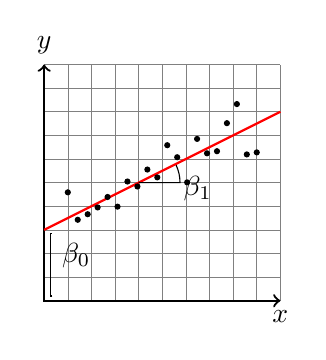
\begin{tikzpicture}[scale=0.15]
\draw[step=2, gray, very thin] (-10,-10) grid (10,10); % background grid
\draw[thick, <->] (-10,10) node[anchor=south] {$y$} -- (-10,-10) -- (10,-10) node[anchor=north] {$x$}; %axis
\draw[red, thick] plot [domain=-10:10] (\x,{1 + 0.5 * \x}); % regression line
\draw plot [only marks, mark=*, mark size=6, domain=-8:8, samples=20] (\x,{rnd * 5 - 1.5 + 0.5 * \x}); % data points
\draw (-9.3,-9.6) -- (-9.5,-9.6) -- (-9.5,-4.3) -- (-9.3, -4.3) node[anchor=north west] {$\beta_0$}; % beta0
\draw (-2,0) -- (1.5,0) arc (0:25:3.5); % beta1 arc
\draw (3,-0.5) node {$\beta_1$}; % beta1
\end{tikzpicture}

\columnbreak

Equation:\\ $y_i = \beta_0 + \beta_1 x_{1i} + u_i$

\vspace*{1mm}

Estimation:\\ $\hat{y}_i = \hat{\beta}_0 + \hat{\beta}_1 x_{1i}$

\vspace*{1mm}

Where: \\ $\hat{\beta}_0 = \overline{y} - \hat{\beta}_1 \overline{x}$ \\ $\hat{\beta}_1 = \frac{Cov(y, x)}{Var(x)}$

\end{multicols}

\subsection*{Multiple regression model}

\setlength{\multicolsep}{0pt} % reduce vertical spacing betwen subsection and multicols
\setlength{\columnsep}{-40pt} % reduce spacing between columns
\begin{multicols}{2} % set columns to 2

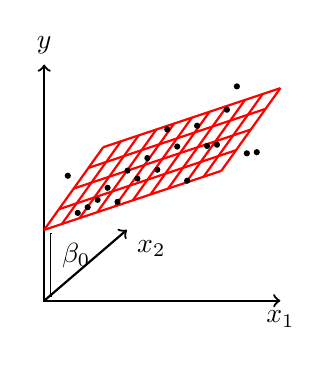
\begin{tikzpicture}[scale=0.15]
\draw[thick, ->] (-10,-10) -- (-3,-4) node[anchor=north west] {$x_2$}; % x2 axis
\draw[thick, <->] (-10,10) node[anchor=south] {$y$} -- (-10,-10) -- (10,-10) node[anchor=north] {$x_1$}; % y and x1 axis
% regression grid
\draw[red, thick] (-10,-4) -- (-5,3);
\draw[red, thick] (-8.5, -3.5) -- (-3.5,3.5);
\draw[red, thick] (-7, -3) -- (-2,4);
\draw[red, thick] (-5.5, -2.5) -- (-0.5,4.5);
\draw[red, thick] (-4, -2) -- (1,5);
\draw[red, thick] (-2.5, -1.5) -- (2.5,5.5);
\draw[red, thick] (-1, -1) -- (4,6);
\draw[red, thick] (0.5, -0.5) -- (5.5,6.5);
\draw[red, thick] (2, 0) -- (7,7);
\draw[red, thick] (3.5, 0.5) -- (8.5,7.5);
\draw[red, thick] (5, 1) -- (10,8);
\draw[red, thick] (-10, -4) -- (5, 1);
\draw[red, thick] (-8.75, -2.25) -- (6.25,2.75);
\draw[red, thick] (-7.5, -0.5) -- (7.5,4.5);
\draw[red, thick] (-6.25, 1.25) -- (8.75,6.25);
\draw[red, thick] (-5,3) -- (10,8);
\draw plot [only marks, mark=*, mark size=6, domain=-8:8, samples=20] (\x,{rnd * 6.5 - 1.5 + 0.5 * \x}); % data points
\draw (-9.3,-9.6) -- (-9.5,-9.6) -- (-9.5,-4.3) -- (-9.3, -4.3) node[anchor=north west] {$\beta_0$}; % beta0
\end{tikzpicture}

\columnbreak

Equation: \\ $y_i = \beta_0 + \beta_1 x_{1i} + ... + \beta_k x_{ki} + u_i$

\vspace*{1mm}

Estimation: \\ $\hat{y}_i = \hat{\beta}_0 + \hat{\beta}_1 x_{1i} + ... + \hat{\beta}_k x_{ki}$

\vspace*{1mm}

Where: \\ $\hat{\beta}_0 = \overline{y} - \hat{\beta}_1 \overline{x}_1 - ... - \hat{\beta}_k \overline{x}_k$ \\ $\hat{\beta}_j = \frac{Cov(y, \text{residualized } x_j)}{Var(\text{residualized } x_j)}$

\vspace*{1mm}

Matrix: $\hat{\beta} = (X^T X)^{-1} (X^T y)$

\end{multicols}

\subsection*{Interpretation of coefficients}

\scalebox{0.872}{ % scale the table to fit in the column
\begin{tabular}{ c c c c }
	Model & Dependent & Independent & $\beta_1$ interpretation \\
	\hline
	Level-level & $y$ & $x$ & $\Delta y = \beta_1 \Delta x$ \\ 
	Level-log & $y$ & $log(x)$ & $\Delta y = (\beta_1/100) \% \Delta x$ \\  
	Log-level & $log(y)$ & $x$ & $\% \Delta y = (100 \beta_1) \Delta x$ \\
	Log-log & $log(y)$ & $log(x)$ & $\% \Delta y = \beta_1 \% \Delta x$ \\
	Quadratic & $y$ & $x + x^2$ & $\Delta y = (\beta_1 + 2 \beta_2 x) \Delta x$ \\
\end{tabular}
}

\subsection*{Error measures}

Sum of Sq. Resid.: \hfill $SSR = \sum_{i=1}^n \hat{u}_i^2 = \sum_{i=1}^n (y_i - \hat{y}_i)^2$

\vspace*{0.5mm}

Expl. Sum of Sq.: \hfill $SSE = \sum_{i=1}^n (\hat{y}_i - \overline{y})^2$

\vspace*{0.5mm}

Tot. Sum of Sq.: \hfill $SST = SSE + SSR = \sum_{i=1}^n (y_i - \overline{y})^2$

\vspace*{0.5mm}

Standard Error of the Regression: \hfill $\hat{\sigma} = \sqrt{\frac{SSR}{n-k-1}}$

\vspace*{0.5mm}

Standard Error of the $\hat{\beta}$'s: \hfill $se(\hat{\beta}) = \hat{\sigma} \sqrt{(X^T X)^{-1}}$

\vspace*{0.5mm}

Sqrt. of the Quadratic Mean Error: \hfill $\sqrt{\frac{\sum_{i=1}^n (\hat{u}_i - \overline{u})^2}{n}}$

\vspace*{0.5mm}

Absolute Mean Error: \hfill $\frac{\sum_{i=1}^n |\hat{u}_i|}{n}$

\vspace*{0.5mm}

Mean Percentage Error: \hfill $\frac{\sum_{i=1}^n |\hat{u}_i / y_i|}{n} \times 100$

\columnbreak

\section*{R-squared}

Is a \textbf{measure of the goodness of the fit}, how the regression fits to the data:

\begin{center}
$R^2 = \frac{SSE}{SST} = 1 - \frac{SSR}{SST}$
\end{center}

\begin{itemize}[leftmargin=*]
\item Measures the \textbf{percentage of variation of $y$ that is linearly explained by the variations of $x$'s}.
\item Takes values \textbf{between 0} (no linear explanation of the variations of $y$) \textbf{and 1} (total explanation of the variations of $y$).
\end{itemize}

When the number of regressors increment, the value of the r-squared increments as well, whatever the new variables are relevant or not. To solve this problem, there is an \textbf{r-squared corrected by degrees of freedom}:

\begin{center}
$\overline{R}^2 = 1 - \frac{n-1}{n-k-1} \frac{SSR}{SST} = 1 - \frac{n-1}{n-k-1} (1-R^2)$
\end{center}

For big sample sizes: $\overline{R}^2 \approx R^2$

\section*{Hypothesis testing}
\subsection*{The basics of hypothesis testing}

An hypothesis test is a rule designed to explain from a sample, if \textbf{exist evidence or not to reject an hypothesis} that is made about one or more population parameters.

Elements of an hypothesis contrast:

\begin{itemize}[leftmargin=*]
\item \textbf{Null hypothesis ($H_0$)} - is the hypothesis to be tested.
\item \textbf{Alternative hypothesis ($H_1$)} - is the hypothesis that cannot be rejected when the null hypothesis is rejected.
\item \textbf{Statistic of contrast}: is a random variable whose probability distribution is known under the null hypothesis and is tabulated.
\item \textbf{Significance level ($\alpha$)} - is the probability of rejecting the null hypothesis being true (type I error). Is chosen by who conduct the contrast. Commonly is 0.10, 0.05, 0.01 or 0.001.
\item \textbf{Critic value} - is the value against which
the statistic of contrast is compared to determine if the
null hypothesis is rejected or not.
\item \textbf{p-value} - is the highest level of significance by which the null hypothesis cannot be rejected ($H_0$).
\end{itemize}

\textbf{The rule is}: if the p-value is less than $\alpha$, there is evidence that, at a given $\alpha$, the null hypothesis is rejected (the alternative is accepted instead).

\subsection*{Individual contrasts}

Tests if a given parameter is significantly different from a given value $\theta$.

\begin{itemize}[leftmargin=*]
\item $H_0: \beta_j = \theta$
\item $H_1: \beta_j \neq \theta$
\end{itemize}

Under $H_0$:

\begin{center}
$t = \frac{\hat{\beta}_j - \theta}{se(\hat{\beta}_j)} \sim t_{n-k-1, \alpha/2}$
\end{center}

If $\mid t \mid > t_{n-k-1, \alpha/2}$ there is evidence to reject the null hypothesis.

\textbf{Individual significance test} - tests if a given parameter is significantly \textbf{different from zero}.

\begin{itemize}[leftmargin=*]
\item $H_0: \beta_j = 0$
\item $H_1: \beta_j \neq 0$
\end{itemize}

Under $H_0$:

\begin{center}
$t = \frac{\hat{\beta}_j}{se(\hat{\beta}_j)} \sim t_{n-k-1, \alpha/2}$
\end{center}

If $\mid t \mid > t_{n-k-1, \alpha/2}$ there is evidence to reject the null hypothesis.

\subsection*{The F contrast}

Simultaneously contrasts multiple (linear) hypothesis about the parameters. It makes use of a non restricted model and a restricted model:

\begin{itemize}[leftmargin=*]
\item \textbf{Non restricted model} - is the model on which we want to test the hypothesis.
\item \textbf{Restricted model} - is the model on which the hypothesis that we want to contrast have been imposed.
\end{itemize}

Then, looking at the errors, there are:

\begin{itemize}[leftmargin=*]
\item \textbf{$\sum_{i=1}^n \hat{u}_{nr}^2$} - is the Sum of Sq. Resid. of the non restricted model ($SSR_{nr}$).
\item \textbf{$\sum_{i=1}^n \hat{u}_r^2$} - is the Sum of Sq. Resid of the restricted model ($SSR_r$).
\end{itemize}

Under $H_0$:

\begin{center}
$F = \frac{SSR_r - SSR_{nr}}{SSR_{nr}} \frac{(n-k_{nr}-1)}{q} \sim F_{q, n-k_{nr}-1}$
\end{center}

Where $k_{nr}$ is the number of parameters of the non restricted model and $q$ is the number of linear hypothesis tested.

If $F_{q, n-k_{nr}-1} < F$, there is evidence to reject the null hypothesis.

\textbf{Global significance test} - tests if all the parameters associated to $x$'s of the model are simultaneously equal to zero or not.

$H_0: \beta_1 = \beta_2 = ... = \beta_k = 0$

$H_1: \beta_1 \neq 0$ and/or $\beta_2 \neq 0 ...$ and/or $\beta_k \neq 0$

If $F_{k, n-k_{nr}-1} < F$, there is evidence to reject the null hypothesis.

\section*{Confidence intervals}

The confidence intervals at ($1 - \alpha$) confidence level can be calculated:

\begin{center}
$\hat{\beta}_j \mp t_{n-k-1, \alpha/2} se(\hat{\beta}_j)$
\end{center}

\section*{Dummy variables and structural change}

Dummy (or binary) variables are used for qualitative information like sex, civil state, country, etc.

\begin{itemize}[leftmargin=*]
\item Get the \textbf{value of 1 in a given category, and 0 on the rest}.
\item Are used to analyze and modeling \textbf{structural changes} in the model parameters.
\end{itemize}

If a qualitative variable have $m$ categories, we only have to include ($m-1$) dummy variables.

\subsection*{Structural change}

Structural change refers to changes in the values of the parameters of the econometric model produced by the effect of different sub-populations. Structural change can be included in the model through dummy variables.

The position of the dummy variable matters:
\begin{itemize}[leftmargin=*]
\item \textbf{On the intercept ($\beta_0$)} - represents the mean difference between the values produced by the structural change.
\item \textbf{On the parameters that determines the slope of the regression line ($\beta_j$)} - represents the effect (slope) difference between the values produced by the structural change.
\end{itemize}

\textbf{The Chow's structural contrast} - when we want to analyze the existence of structural changes in all the model parameters, it is common to use a particular expression of the F contrast known as the Chow's contrast, where the null hypothesis is: $H_0: \text{No structural change}$

\section*{Predictions}

Two types of prediction:

\begin{itemize}[leftmargin=*]
\item Of the mean value of $y$ for a specific value of $x$.
\item Of an individual value of $y$ for a specific value of $x$.
\end{itemize}

If the values of the variables ($x$) approximate to the mean values ($\overline{x}$), the confidence interval amplitude of the prediction will be shorter. 

\columnbreak

\section*{Multicollinearity}

\begin{itemize}[leftmargin=*]
\item \textbf{Perfect multicollinearity} - there are independent variables that are constant and/or there is an exact linear relation between independent variables. Is the \textbf{breaking of the third (3) econometric model assumption}.
\item \textbf{Approximate multicollinearity} - there are independent variables that are approximately constant and/or there is an approximately linear relation between independent variables. It \textbf{does not break any econometric model assumption}, but has an effect on OLS.
\end{itemize}

\subsection*{Consequences}

\begin{itemize}[leftmargin=*]
\item \textbf{Perfect multicollinearity} - the equation system of OLS cannot be solved due to infinite solutions.
\item \textbf{Approximate multicollinearity}
\begin{itemize}[leftmargin=*]
\item Small sample variations can induce to big variations in the OLS estimations.
\item The variance of the OLS estimators of the $x$'s that are collinear, increments, thus the inference of the parameter is affected. The estimation of the parameter is very imprecise (big confidence interval).
\end{itemize}
\end{itemize}

\subsection*{Detection}

\begin{itemize}[leftmargin=*]
\item \textbf{Correlation analysis} - look for high correlations (greater than 0.7) between independent variables.
\item \textbf{Variance Inflation Factor (VIF)} - indicates the increment of $Var(\hat{\beta}_j)$ because of the multicollinearity.
\begin{center}
$VIF(\hat{\beta}_j) = \frac{1}{1-R_j^2}$
\end{center}
Where $R^2_j$ denotes the r-squared from a regression between $x_j$ and all the other $x$'s. 
\begin{itemize}[leftmargin=*]
\item Values between 4 to 10 suggest that it is advisable to analyze in more depth if there might be multicollinearity problems.
\item Values bigger than 10 indicates that there are multicollinearity problems.
\end{itemize}
\end{itemize}

One typical characteristic of multicollinearity is that the regression coefficients of the model are not individually different from zero (due to high variances), but jointly they are different from zero.

\subsection*{Correction}

\begin{itemize}[leftmargin=*]
\item Delete one of the collinear variables.
\item Perform factorial analysis (or any other dimension reduction technique) on the collinear variables.
\item Interpret coefficients with multicollinearity jointly.
\end{itemize}

\columnbreak

\section*{Heteroscedasticity}

The residuals $u_i$ of the population regression function do not have the same variance $\sigma^2$:

\begin{center}
$Var(u|x) = Var(y|x) \neq \sigma^2$
\end{center}

Is the \textbf{breaking of the fifth (5) econometric model assumption}.

\subsection*{Consequences}

\begin{itemize}[leftmargin=*]
\item OLS estimators still are unbiased.
\item OLS estimators still are consistent.
\item OLS is \textbf{not efficient} anymore, but still a LUE (Linear Unbiased Estimator).
\item \textbf{Variance estimations of the estimators is biased}: the construction of confidence intervals and the hypothesis contrast are not reliable.
\end{itemize}

\subsection*{Detection}

\begin{itemize}[leftmargin=*]
\setlength{\multicolsep}{0pt} % reduce vertical spacing betwen subsection and multicols
\setlength{\columnsep}{20pt} % increment spacing between columns
\begin{multicols}{3} % set columns to 3
\item \textbf{Graphical analysis} - look for scatter patterns on $x$ vs. $u$ or $x$ vs. $y$ plots.

\columnbreak

\vspace*{-23pt}

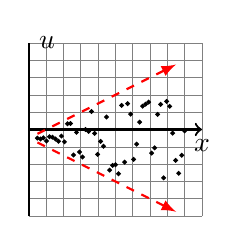
\begin{tikzpicture}[scale=0.11]
\draw[step=2, gray, very thin] (-10,-10) grid (10,10); % grid
\draw[thick,->] (-10,0) -- (10,0) node[anchor=north] {$x$}; % x axis
\draw[thick,-] (-10,-10) -- (-10,10) node[anchor=west] {$u$}; % u axis
\draw plot [only marks, mark=*, mark size=6, domain=0:17, samples=50] ({\x - 9},{-0.5 * rand * \x - 1}); % data points
\draw[thick, dashed, red, -latex] plot [domain=1:17] ({\x - 10},{-0.5 * \x - 1}); % lower red arrow
\draw[thick, dashed, red, -latex] plot [domain=1:17] ({\x - 10},{0.5 * \x - 1}); % upper red arrow
\end{tikzpicture}

\columnbreak

\vspace*{-24pt}

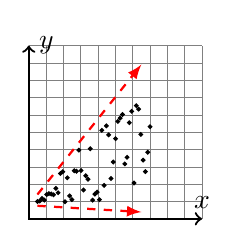
\begin{tikzpicture}[scale=0.11]
\draw[step=2, gray, very thin] (-10,-10) grid (10,10); % grid
\draw[thick,<->] (-10,10) node[anchor=west] {$y$} -- (-10,-10) -- (10,-10) node[anchor=south] {$x$}; % axis
\draw plot [only marks, mark=*, mark size=6, domain=0:13, samples=50] ({\x -9},{(-0.65 * rand * \x) + 0.6 * \x - 8}); % data points
\draw[thick, dashed, red, -latex] plot [domain=0:12] ({\x - 9},{-0.06 * \x - 8.5}); % lower red arrow
\draw[thick, dashed, red, -latex] plot [domain=0:12] ({\x -9},{1.25 * \x - 7.2}); % upper red arrow
\end{tikzpicture}

\end{multicols}

\item \textbf{Formal tests} - White, Bartlett, Breusch-Pagan, etc. Commonly, the null hypothesis: $H_0 = \text{Homoscedasticity}$
\end{itemize}

\subsection*{Correction}

\begin{itemize}[leftmargin=*]
\item Use OLS with a variance-covariance matrix estimator robust to heteroscedasticity, for example, the one proposed by White.
\item If the variance structure is known, make use of Weighted Least Squares (WLS) or Generalized Least Squares (GLS).
\item If the variance structure is not known, make use of Feasible Weighted Least Squared (FWLS), that estimates a possible variance, and divides the model variables by it and then apply OLS.
\item Make assumptions about the possible variance:
\begin{itemize}[leftmargin=*]
\item Supposing that $\sigma_i^2$ is proportional to $x_i$, divide the model variables by the square root of $x_i$ and apply OLS.
\item Supposing that $\sigma_i^2$ is proportional to $x_i^2$, divide the model variables by $x_i$ and apply OLS.
\end{itemize}
\item Make a new model specification, for example, logarithmic transformation.
\end{itemize}

\columnbreak

\section*{Auto-correlation}

The residual of any observation, $u_t$, is correlated with the residual of any other observation. The observations are not independent.

\begin{center}
$Corr(u_t, u_s | x) \neq 0$ for any $t \neq s$
\end{center}

The ``natural" context of this phenomena is in temporal series. Is the \textbf{breaking of the sixth (6) econometric model assumption}.

\subsection*{Consequences}

\begin{itemize}[leftmargin=*]
\item OLS estimators still are unbiased.
\item OLS estimators still are consistent.
\item OLS is \textbf{not efficient} anymore, but still a LUE (Linear Unbiased Estimator).
\item \textbf{Variance estimations of the estimators is biased}: the construction of confidence intervals and the hypothesis contrast are not reliable.
\end{itemize}

\subsection*{Detection}

\begin{itemize}[leftmargin=*]
\item \textbf{Graphical analysis} - look for scatter patterns on $u_{t-1}$ vs. $u_t$ or make use of a correlogram.

\setlength{\multicolsep}{0pt} % reduce vertical spacing betwen subsection and multicols
\setlength{\columnsep}{6pt} % increment spacing between columns
\begin{multicols}{3} % set columns to 3

\begin{center}
\textbf{\footnotesize AR}
\end{center}

\vspace{2.0pt}

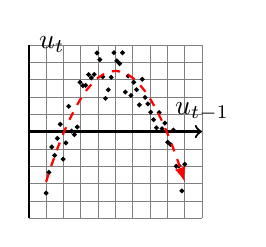
\begin{tikzpicture}[scale=0.11]
\draw[step=2, gray, very thin] (-10,-10) grid (10,10); % grid
\draw[thick,->] (-10,0) -- (10,0) node[anchor=south] {$u_{t-1}$}; % ut-1 axis
\draw[thick,-] (-10,-10) -- (-10,10) node[anchor=west] {$u_t$}; % ut axis
\draw plot [only marks, mark=*, mark size=6, domain=-8:8, samples=50] (\x,{rnd * 6 + (-2 * (\x)^2 + 40) * 0.1}); % data points
\draw[thick, dashed, red, -latex] plot [domain=-8:8] (\x,{3 + (-2 * (\x)^2 + 40) * 0.1}); % red arrow
\end{tikzpicture}

\columnbreak

\begin{center}
\textbf{\footnotesize AR(+)}
\end{center}

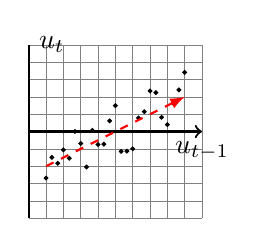
\begin{tikzpicture}[scale=0.11]
\draw[step=2, gray, very thin] (-10,-10) grid (10,10); % grid
\draw[thick,->] (-10,0) -- (10,0) node[anchor=north] {$ u_{t-1}$}; % ut-1 axis
\draw[thick,-] (-10,-10) -- (-10,10) node[anchor=west] {$u_t$}; % ut axis
\draw plot [only marks, mark=*, mark size=6, domain=-8:8, samples=25] (\x,{rnd * 6 + 0.5 * \x - 3}); % data points
\draw[thick, dashed, red, -latex] plot [domain=-8:8] (\x,{3 + 0.5 * \x - 3}); % red arrow
\end{tikzpicture}

\columnbreak

\begin{center}
\textbf{\footnotesize AR(-)}
\end{center}

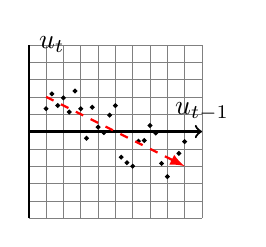
\begin{tikzpicture}[scale=0.11]
\draw[step=2, gray, very thin] (-10,-10) grid (10,10); % grid
\draw[thick,->] (-10,0) -- (10,0) node[anchor=south] {$u_{t-1}$}; % ut-1 axis
\draw[thick,-] (-10,-10) -- (-10,10) node[anchor=west] {$u_t$}; % ut axis
\draw plot [only marks, mark=*, mark size=6, domain=-8:8, samples=25] (\x,{rnd * 6 - 0.5 * \x - 3}); % data points
\draw[thick, dashed, red, -latex] plot [domain=-8:8] (\x,{3 - 0.5 * \x - 3}); % red arrow
\end{tikzpicture}

\end{multicols}

\item \textbf{Formal tests} - Durbin-Watson, Breusch-Godfrey, etc. Commonly, the null hypothesis: $H_0: \text{No auto-correlation}$

\end{itemize}

\subsection*{Correction}

\begin{itemize}[leftmargin=*]
\item Use OLS with a variance-covariance matrix estimator robust to auto-correlation, for example, the one proposed by Newey-West.
\item Use Generalized Least Squares. Supposing $y_t = \beta_0 + \beta_1 x_t + u_t$, with $u_t = \rho u_{t-1} + \varepsilon_t$, where $|\rho| < 1$ and $\varepsilon_t$ is white noise.
\begin{itemize}[leftmargin=*]
\item If $\rho$ is known, create a quasi-differentiated model where $u_t$ is white noise and estimate it by OLS.
\item If $\rho$ is not known, estimate it by -for example- the Cochrane-Orcutt method, create a quasi-differentiated model where $u_t$ is white noise and estimate it by OLS.
\end{itemize}
\end{itemize}

\end{multicols}
\end{document}